% This file was created by tikzplotlib v0.9.8.
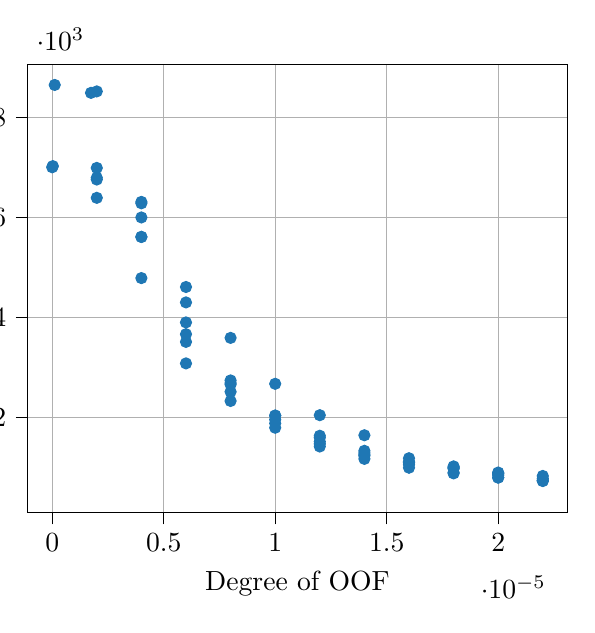
\begin{tikzpicture}[trim axis left,trim axis right]

\definecolor{color0}{rgb}{0.12156862745098,0.466666666666667,0.705882352941177}

\begin{axis}[
scaled y ticks=base 10:-3,
legend cell align={left},
legend style={fill opacity=0.8, draw opacity=1, text opacity=1, draw=white!80!black},
tick align=outside,
tick pos=left,
% title={Feature count vs. OOF},
x grid style={white!69.0196078431373!black},
xlabel={Degree of OOF},
xmin=-1.09892007559144e-06, xmax=2.31000189170211e-05,
xtick style={color=black},
xmajorgrids,
ymajorgrids,
y grid style={white!69.0196078431373!black},
ylabel={\# features},
ymin=99.9931235536055, ymax=9059.85673521721,
ytick style={color=black},
% y tick label style={/pgf/number format/sci}
]
\addplot [draw=color0, fill=color0, forget plot, mark=*, only marks]
table{%
x  y
2.89713740402389e-08 7023
1.79997717738205e-05 977
9.99997577071001e-06 1882
2.00011560321043e-06 6755
6.00014606118044e-06 4607
1.20001917481398e-05 2045
2.19998022317905e-05 743
1.99991485475958e-06 6791
3.99993008374979e-06 5606
5.99994531274e-06 3664
1.80000366866596e-05 899
2.00000519156498e-05 798
8.00016129016978e-06 3590
1.000017651916e-05 2672
1.400020697713e-05 1644
1.99997870028003e-05 874
7.99996054173021e-06 2513
1.40000062286896e-05 1233
1.60002222061202e-05 1185
1.19999909997002e-05 1419
1.60000214576702e-05 1056
4.00013083219977e-06 5610
2.20000671446296e-05 728
1.400020697713e-05 1172
3.99993008374979e-06 6308
7.99996054173021e-06 2688
9.99997577071001e-06 2037
1.03169680003984e-09 7000
1.000017651916e-05 1794
2.19998022317905e-05 741
1.99991485475958e-06 6987
5.99994531274e-06 4299
1.40000062286896e-05 1291
1.80000366866596e-05 988
2.00011560321043e-06 6389
4.00013083219977e-06 4785
6.00014606118044e-06 3080
8.00016129016978e-06 2329
1.20001917481398e-05 1472
1.60002222061202e-05 995
1.79997717738205e-05 882
1.19999909997002e-05 1595
1.60000214576702e-05 1103
2.00000519156498e-05 847
2.20000671446296e-05 781
1.99997870028003e-05 798
1.14187389609749e-07 8645
1.74120792746993e-06 8487
4.00013083219977e-06 5997
2.19998022317905e-05 831
1.99991485475958e-06 8516
3.99993008374979e-06 6280
9.99997577071001e-06 2037
1.80000366866596e-05 1004
6.00014606118044e-06 3510
8.00016129016978e-06 2658
1.20001917481398e-05 1517
1.60002222061202e-05 1095
7.99996054173021e-06 2740
2.00000519156498e-05 888
1.000017651916e-05 1958
1.79997717738205e-05 1022
1.99997870028003e-05 899
1.19999909997002e-05 1634
1.40000062286896e-05 1333
1.60000214576702e-05 1118
1.400020697713e-05 1253
5.99994531274e-06 3899
};
% \addplot [semithick, red]
% table {%
% 1.03169680003984e-09 8652.59020741432
% 2.89713740402389e-08 8621.47458132233
% 1.14187389609749e-07 8527.26131703851
% 1.74120792746993e-06 6913.51092038955
% 1.99991485475958e-06 6686.69355019204
% 1.99991485475958e-06 6686.69355019204
% 1.99991485475958e-06 6686.69355019204
% 2.00011560321043e-06 6686.52046851991
% 2.00011560321043e-06 6686.52046851991
% 3.99993008374979e-06 5166.70076818288
% 3.99993008374979e-06 5166.70076818288
% 3.99993008374979e-06 5166.70076818288
% 4.00013083219977e-06 5166.56703075379
% 4.00013083219977e-06 5166.56703075379
% 4.00013083219977e-06 5166.56703075379
% 5.99994531274e-06 3992.22674518632
% 5.99994531274e-06 3992.22674518632
% 5.99994531274e-06 3992.22674518632
% 6.00014606118044e-06 3992.1234084266
% 6.00014606118044e-06 3992.1234084266
% 6.00014606118044e-06 3992.1234084266
% 7.99996054173021e-06 3084.72952084398
% 7.99996054173021e-06 3084.72952084398
% 7.99996054173021e-06 3084.72952084398
% 8.00016129016978e-06 3084.6496741889
% 8.00016129016978e-06 3084.6496741889
% 8.00016129016978e-06 3084.6496741889
% 9.99997577071001e-06 2383.52098318378
% 9.99997577071001e-06 2383.52098318378
% 9.99997577071001e-06 2383.52098318378
% 1.000017651916e-05 2383.45928695194
% 1.000017651916e-05 2383.45928695194
% 1.000017651916e-05 2383.45928695194
% 1.19999909997002e-05 1841.70840227035
% 1.19999909997002e-05 1841.70840227035
% 1.19999909997002e-05 1841.70840227035
% 1.20001917481398e-05 1841.66073058486
% 1.20001917481398e-05 1841.66073058486
% 1.20001917481398e-05 1841.66073058486
% 1.40000062286896e-05 1423.05851843724
% 1.40000062286896e-05 1423.05851843724
% 1.40000062286896e-05 1423.05851843724
% 1.400020697713e-05 1423.02168329095
% 1.400020697713e-05 1423.02168329095
% 1.400020697713e-05 1423.02168329095
% 1.60000214576702e-05 1099.57447357174
% 1.60000214576702e-05 1099.57447357174
% 1.60000214576702e-05 1099.57447357174
% 1.60002222061202e-05 1099.54601164414
% 1.60002222061202e-05 1099.54601164414
% 1.60002222061202e-05 1099.54601164414
% 1.79997717738205e-05 849.652567006649
% 1.79997717738205e-05 849.652567006649
% 1.79997717738205e-05 849.652567006649
% 1.80000366866596e-05 849.623544825807
% 1.80000366866596e-05 849.623544825807
% 1.80000366866596e-05 849.623544825807
% 1.99997870028003e-05 656.512899491502
% 1.99997870028003e-05 656.512899491502
% 1.99997870028003e-05 656.512899491502
% 2.00000519156498e-05 656.490474517362
% 2.00000519156498e-05 656.490474517362
% 2.00000519156498e-05 656.490474517362
% 2.19998022317905e-05 507.276978773357
% 2.19998022317905e-05 507.276978773357
% 2.19998022317905e-05 507.276978773357
% 2.20000671446296e-05 507.259651356497
% 2.20000671446296e-05 507.259651356497
% };
% \addlegendentry{\#features $\approx 8653.74e^{-128941.61x}$}
\end{axis}

\end{tikzpicture}
